\section{Transcodificação de Vídeo}
\label{cap:2.1}

A modificação do \textit{bitstream} de vídeo codificado é uma prática comum na indústria e visa sanar as mais diversas necessidades. Uma delas é a migração de vídeos codificados com tecnologias mais antigas para tecnologias mais recentes e mais eficientes em termos de compressão de dados. Outra é permitir que uma transmissão seja compatível com os mais diversos reprodutores de vídeo disponíveis no mercado, o que só é possível se o transmissor do vídeo disponibilizar \textit{bitstream}s para os mais diversos formatos. Essas e tantas outras necessidades são satisfeitas através do uso de um transcodificador de vídeo. O funcionamento básico da transcodificação de vídeo, conforme ilustrado na Figura \ref{fig:3}, pode ser resumido em um processo em cascata no qual um vídeo codificado com a tecnologia antiga (OLD) é decodificado e recodificado com uma tecnologia nova (NEW). Esse modelo geral de transcodificação de vídeo, também denominado como transcodificador em cascata, ou típico, ou ainda original (inclusive, este último será utilizado no decorrer da tese), não é exclusivo de formatos digitais, já sendo utilizado desde o advento de transmissão comercial de programas de televisão, no qual a migração de sinais analógicos de vídeos já era comum. Isso pode ser visto em \cite{bib:transcoding67}, quem propôs uma solução em hardware capaz de modificar o sinal de vídeos originários da Europa Ocidental para se adequarem aos televisores norte-americanos, já que a frequência eletromagnética e a organização das linhas de raios catódicos dos televisores eram divergentes entre as duas regiões.

\begin{figure}
    \centering
    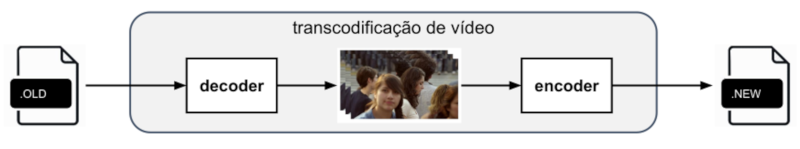
\includegraphics[width=\textwidth]{FIGURES/fig_3.png}
    \caption{Visão em alto nível de um transcodificador de vídeo original. Fonte: Elaborada pelo autor.}
    \label{fig:3}
\end{figure}

Atualmente, na era das tecnologias digitais, há dois tipos fundamentais de transcodificadores: heterogêneos e homogêneos. Eles são facilmente identificados ao se observar quais são os formatos utilizados em uma transcodificação: caso OLD e NEW sejam iguais, trata-se de uma transcodificação homogênea; caso contrário, uma transcodificação heterogênea. Apesar da transcodificação homogênea não envolver troca no formato de codificação, é muito utilizada pela indústria de vídeos, de modo a atingir algum objetivo particular, como a redução da taxa de bits por segundo, redução da resolução, adaptação do \textit{bitstream} para diferentes configurações temporais, inserção de marca d’água, etc. Em \citet{bib:modosTranscodificacao}, o autor identificou diversas utilizações de um transcodificador de vídeo, vide Figura \ref{fig:4}.

\begin{figure}
    \centering
    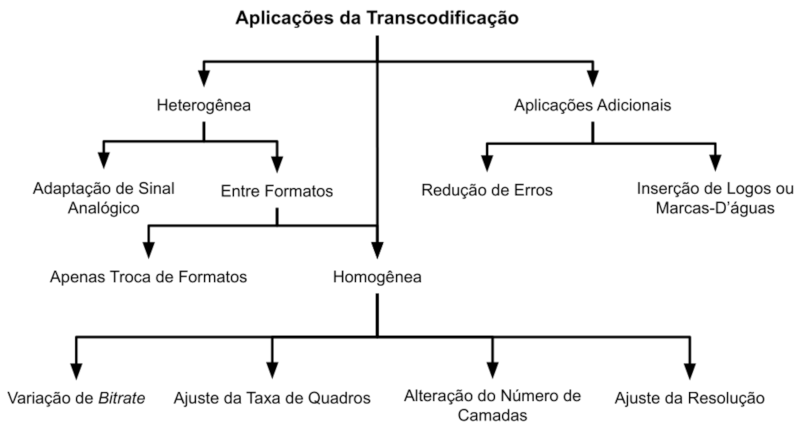
\includegraphics[width=\textwidth]{FIGURES/fig_4.png}
    \caption{Classificação de transcodificadores de vídeo. Fonte: Elaborada pelo autor com base em \citet{bib:modosTranscodificacao}.}
    \label{fig:4}
\end{figure}

Na literatura científica, a transcodificação homogênea é apresentada, principalmente, como solução para a redução da taxa de bits do vídeo (também identificado como \textit{transrating}), como no trabalho de \citet{bib:nam_2006}, mas também para a redução da resolução do vídeo, como em \citet{bib:nguyen_2015}. Esta última modalidade, que pode ser identificada como \textit{downscaling}, visa adequar a resolução original do vídeo para os mais diversos meios de reprodução que o usuário possa utilizar, já que, quando a resolução do vídeo é reduzida, a taxa de bits também o é. A preocupação com a redução do tamanho do \textit{bitstream} de forma a se adequar à largura de banda na transmissão de vídeo pode ser observada desde os princípios da internet, como pode ser visto nos trabalhos de \citet{bib:shen_1997} e \citet{bib:swann_1996}, que propuseram soluções de transcodificação para adequar o \textit{bitstream} a diferentes meios de transmissão de dados, de forma a apresentar o menor erro possível na transmissão do vídeo e manter a experiência do usuário relativamente adequada. Como na transcodificação homogênea o software codificador opera com o mesmo formato de codificação que o decodificador, a diferença entre as versões do \textit{bitstream} está em particularidades da codificação, isto é, nas configurações utilizadas.

Já a transcodificação heterogênea visa de fato a mudança no formato de codificação de vídeo usado. Uma das principais razões para se aplicar esse tipo de transcodificação é permitir a compatibilidade de um vídeo com diferentes sistemas de reprodução. Em outras palavras, um vídeo codificado com tecnologias recentes que precisa ser reproduzido em sistemas antigos (\textit{backward compatibility}) ou um vídeo codificado com tecnologias antigas que precisa ser atualizado para reprodução em sistemas mais recentes (\textit{forward compatibility}). Outros motivos, como a existência de políticas de royalties associadas à reprodução de vídeos em certos formatos, também podem motivar a conversão entre formatos. A existência de múltiplos sistemas de reprodução de vídeo no mundo real é também uma razão para que empresas necessitem manter seus vídeos em mais de um formato de codificação, como é o caso do YouTube, que oferece suporte simultaneamente aos formatos H.264, VP9 e AV1 \cite{bib:bitmovin_ott_report_2020} \cite{bib:5to9google}.

Por fim, como mostra a Figura \ref{fig:4}, também há uma categoria de transcodificação para aplicações adicionais, que não busca realizar uma modificação do \textit{bitstream} propriamente dita, mas apenas incluir nele funcionalidades novas, como inserção de marca-d'água, legendas (embutidas ou não), novas opções de idioma, etc. Normalmente esse tipo de transcodificação não é comum na literatura científica, mas pode-se citar o trabalho de \citet{bib:watermark}, que visa remover marcas-d’água existentes em vídeos.

A correta categorização da transcodificação é útil em duas situações específicas: saber quais parâmetros da codificação devem ser configurados e quais informações são particularmente importantes para serem consideradas durante uma transcodificação de vídeo acelerada. Nesta tese, destacamos principalmente os trabalhos voltados para transcodificações heterogêneas, pois os custos computacionais de execução de um codificador e um decodificador se dão em escalas diferentes. O codificador deve considerar todas as opções disponíveis no formato de codificação a fim de encontrar a melhor combinação de decisões para cada região do vídeo, gerando assim um \textit{bitstream} com a maior eficiência de codificação possível. O decodificador, por sua vez, precisa apenas reverter o \textit{bitstream} em arquivo de vídeo. Logo, havendo a possibilidade de reduzir o custo computacional ao executar o codificador, ela deve ser aproveitada.

Observa-se o emprego de quatro estratégias para realizar a transcodificação rápida:

\begin{itemize}
    \item A partir do reaproveitamento de informações provenientes exclusivamente do decodificador, com soluções baseadas em heurísticas;
    
    \item A partir do reaproveitamento de informações provenientes tanto do decodificador como do codificador, com soluções baseadas em heurísticas;

    \item A partir do reaproveitamento de informações provenientes exclusivamente do decodificador, com soluções baseadas em modelos preditivos treinados por aprendizado de máquina;

    \item A partir do reaproveitamento de informações provenientes tanto do decodificador como do codificador, com soluções baseadas em modelos preditivos treinados por aprendizado de máquina.
\end{itemize}

Apesar de todas as opções acima serem representáveis pela Figura \ref{fig:5}, a origem dos reaproveitamentos na figura leva em conta apenas informações extraídas do decodificador. Todavia, também é possível o reaproveitamento de informações provenientes do próprio codificador.

\begin{figure}
    \centering
    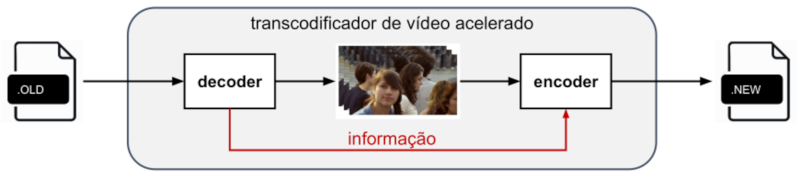
\includegraphics[width=\textwidth]{FIGURES/fig_5.png}
    \caption{Representação em alto nível de uma transcodificação rápida de vídeo. Fonte: Elaborada pelo autor.}
    \label{fig:5}
\end{figure}

Independentemente da classificação de transcodificador rápido que se faz uso, existe, em todas elas, a possibilidade de obter os dados provenientes do processo de decodificação, sendo possível transformá-los em conhecimento sobre o vídeo que será codificado. Portanto, esse conhecimento deve ser utilizado para realizar otimizações no processo decisório da codificação, com o objetivo primário de reduzir o custo computacional de executar a transcodificação e, sempre que possível, com o menor impacto na eficiência de codificação.

Assim sendo, no capítulo \ref{cap:3}, serão apresentados trabalhos publicados na literatura científica que propõem estratégias para acelerar o processo de transcodificação de vídeo. A ideia comum entre eles é o reaproveitamento de informações extraídas da decodificação (e, eventualmente, também do codificador), com ou sem uso de tratamento de dados. Dessa forma, é possível remover total ou parcialmente algumas decisões do codificador, reduzindo seu custo computacional. Para possibilitar essa aceleração, usualmente são implementadas heurísticas que relacionam os dados previamente capturados com a decisão que precisa ser realizada na codificação. Essas heurísticas podem ter, basicamente, dois tipos de embasamento: (1) através de modelos de análises estatísticas e (2) através de modelos preditivos treinados com técnicas de aprendizado de máquina. 

Diferentemente do que ocorre na transcodificação homogênea, na qual a similaridade entre dados extraídos da decodificação e decisões realizadas na recodificação são altamente correlacionados, o que possibilita o desenvolvimento de modelos heurísticos baseados em análises estatísticas de forma mais simplificada, o mesmo não ocorre na transcodificação heterogênea. Logo, um dos principais desafios na aceleração desta envolve o processo de compatibilizar as estruturas de informação e tipos de dados herdados do decodificador e os utilizados pelo codificador. Quanto maior o desafio de compatibilização, maior é a dificuldade de se acelerar um transcodificador baseado em análises estatísticas de forma eficiente. Essa é uma das razões pelas quais trabalhos com ênfase no uso de modelos de aprendizado de máquina para transcodificação de vídeo têm ganhado destaque nos últimos anos, já que esses modelos permitem a descoberta de relações entre um número maior de variáveis de forma mais eficaz que um ser humano. Portanto, na seção \ref{cap:2.2} apresentaremos uma visão geral sobre técnicas de aprendizado de máquina.
